% This template has been tested with IEEEtran of 2015.
% Template from https://github.com/latextemplates/IEEE

% !TeX spellcheck = en-US
% !TeX encoding = utf8
% !TeX program = pdflatex
% !BIB program = bibtex
% -*- coding:utf-8 mod:LaTeX -*-

% To set up:
% aptitude install texlive-publishers texlive-lang-european texlive-latex-extra

%cmap has to be loaded before any font package (such as newtxmath)
\RequirePackage{cmap}

% DO NOT DOWNLOAD IEEEtran.cls - Use the one of your LaTeX distribution
% On Ubuntu, aptitude install texlive-publishers
\documentclass[journal]{IEEEtran}[2015/08/26]

% use nicer font for code
\usepackage[zerostyle=b,scaled=.75]{newtxtt}

\usepackage[T1]{fontenc}
\usepackage[utf8]{inputenc} %support umlauts in the input
% I added the following to get Times Roman in math. Otherwise the g's looked really different.
% See https://tex.stackexchange.com/questions/9685/math-and-times-font#9686
\usepackage[italic]{mathastext}

\usepackage{graphicx}

\usepackage[inkscapelatex=false]{svg}

%Set English as language and allow to write hyphenated"=words
% For Turkish, on Ubuntu aptitude install texlive-lang-european
\usepackage[english]{babel}
% If using Turkish, also set option shorthands=off
%Hint by http://tex.stackexchange.com/a/321066/9075 -> enable "= as dashes
%\addto\extrasenglish{\languageshorthands{ngerman}\useshorthands{"}}

% backticks (`) are rendered as such in verbatim environment. See https://tex.stackexchange.com/a/341057/9075 for details.
\usepackage{upquote}

%extended enumerate, such as \begin{compactenum}
\usepackage{paralist}

%for easy quotations: \enquote{text}
\usepackage{csquotes}

\usepackage{amsmath}

%enable margin kerning
\RequirePackage{iftex}
\ifPDFTeX
  \RequirePackage[%
    final,%
    expansion=alltext,%
    protrusion=alltext-nott]{microtype}%
\else
  \RequirePackage[%
    final,%
    protrusion=alltext-nott]{microtype}%
\fi%
% \texttt{test -- test} keeps the "--" as "--" (and does not convert it to an en dash)
\DisableLigatures{encoding = T1, family = tt* }

%tweak \url{...}
\usepackage{url}
%\urlstyle{same}
%improve wrapping of URLs - hint by http://tex.stackexchange.com/a/10419/9075
\makeatletter
\g@addto@macro{\UrlBreaks}{\UrlOrds}
\makeatother
%nicer // - solution by http://tex.stackexchange.com/a/98470/9075
%DO NOT ACTIVATE -> prevents line breaks
%\makeatletter
%\def\Url@twoslashes{\mathchar`\/\@ifnextchar/{\kern-.2em}{}}
%\g@addto@macro\UrlSpecials{\do\/{\Url@twoslashes}}
%\makeatother

% Diagonal lines in a table - http://tex.stackexchange.com/questions/17745/diagonal-lines-in-table-cell
% Slashbox is not available in texlive (due to licensing) and also gives bad results. This, we use diagbox
%\usepackage{diagbox}

\usepackage{booktabs}

% Required for package pdfcomment later
\usepackage{xcolor}

% For listings
\usepackage{listings}
\lstset{%
  basicstyle=\ttfamily,%
  columns=fixed,%
  basewidth=.5em,%
  xleftmargin=0.5cm,%
  captionpos=b}%

% Enable nice comments
\usepackage{pdfcomment}
%
\newcommand{\commentontext}[2]{\colorbox{yellow!60}{#1}\pdfcomment[color={0.234 0.867 0.211},hoffset=-6pt,voffset=10pt,opacity=0.5]{#2}}
\newcommand{\commentatside}[1]{\pdfcomment[color={0.045 0.278 0.643},icon=Note]{#1}}
%
% Compatibility with packages todo, easy-todo, todonotes
\newcommand{\todo}[1]{\commentatside{#1}}
% Compatiblity with package fixmetodonotes
\newcommand{\TODO}[1]{\commentatside{#1}}

% Bibliopgraphy enhancements
%  - enable \cite[prenote][]{ref}
%  - enable \cite{ref1,ref2}
% Alternative: \usepackage{cite}, which enables \cite{ref1, ref2} only (otherwise: Error message: "White space in argument")
%
% Doc: http://texdoc.net/natbib
\ifCLASSOPTIONcompsoc
  % IEEE Computer Society needs nocompress option at cite.sty
  % natbib includes the same functionality
  \usepackage[%
    square,        % for square brackets
    comma,         % use commas as separators
    numbers,       % for numerical citations;
    sort           % orders multiple citations into the sequence in which they appear in the list of references;
    %sort&compress % as sort but in addition multiple numerical citations
                   % are compressed if possible (as 3-6, 15);
  ]{natbib}
\else
  % normal IEEE
  \usepackage[%
    square,        % for square brackets
    comma,         % use commas as separators
    numbers,       % for numerical citations;
    %sort           % orders multiple citations into the sequence in which they appear in the list of references;
    sort&compress % as sort but in addition multiple numerical citations
                   % are compressed if possible (as 3-6, 15);
  ]{natbib}
\fi
% Same fontsize as without natbib
\renewcommand{\bibfont}{\normalfont\footnotesize}

% Enable hyperlinked author names in the case of \citet
% Source: https://tex.stackexchange.com/a/76075/9075
\usepackage{etoolbox}
\makeatletter
\patchcmd{\NAT@test}{\else \NAT@nm}{\else \NAT@hyper@{\NAT@nm}}{}{}
\makeatother

% Enable that parameters of \cref{}, \ref{}, \cite{}, ... are linked so that a reader can click on the number an jump to the target in the document
\usepackage{hyperref}
% Enable hyperref without colors and without bookmarks
\hypersetup{hidelinks,
  colorlinks=true,
  allcolors=black,
  pdfstartview=Fit,
  breaklinks=true}
%
% Enable correct jumping to figures when referencing
\usepackage[all]{hypcap}

%enable \cref{...} and \Cref{...} instead of \ref: Type of reference included in the link
\usepackage[capitalise,nameinlink]{cleveref}
%\crefname{lstlisting}{\lstlistingname}{\lstlistingname}
%\Crefname{lstlisting}{Listing}{Listings}

%Following definitions are outside of IfPackageLoaded; inside, they are not visible
%
%Intermediate solution for hyperlinked refs. See https://tex.stackexchange.com/q/132420/9075 for more information.
\newcommand{\Vlabel}[1]{\label[line]{#1}\hypertarget{#1}{}}
\newcommand{\lref}[1]{\hyperlink{#1}{\FancyVerbLineautorefname~\ref*{#1}}}

\newenvironment{listing}[1][htbp!]{\begin{figure}[#1]}{\end{figure}}
\newcounter{listing}

\usepackage{xspace}
%\newcommand{\eg}{e.\,g.\xspace}
%\newcommand{\ie}{i.\,e.\xspace}
\newcommand{\eg}{e.\,g.,\ }
\newcommand{\ie}{i.\,e.,\ }

%introduce \powerset - hint by http://matheplanet.com/matheplanet/nuke/html/viewtopic.php?topic=136492&post_id=997377
\DeclareFontFamily{U}{MnSymbolC}{}
\DeclareSymbolFont{MnSyC}{U}{MnSymbolC}{m}{n}
\DeclareFontShape{U}{MnSymbolC}{m}{n}{
  <-6>    MnSymbolC5
  <6-7>   MnSymbolC6
  <7-8>   MnSymbolC7
  <8-9>   MnSymbolC8
  <9-10>  MnSymbolC9
  <10-12> MnSymbolC10
  <12->   MnSymbolC12%
}{}
\DeclareMathSymbol{\powerset}{\mathord}{MnSyC}{180}

% *** SUBFIGURE PACKAGES ***
\ifCLASSOPTIONcompsoc
  \usepackage[caption=false,font=footnotesize,labelfont=sf,textfont=sf]{subfig}
\else
  \usepackage[caption=false,font=footnotesize]{subfig}
\fi

\usepackage{stfloats}



% correct bad hyphenation here
\hyphenation{op-tical net-works semi-conduc-tor}


%\bibliographystyle{chicago}   % For drafts only, to make it easier to see which references have been used.
\bibliographystyle{IEEEtranN} % IEEEtranN is the natbib compatible bst file
%\usepackage{showkeys}          % For drafts only


\begin{document}
%\IEEEoverridecommandlockouts

\title{Operational Optimization of an Agricultural Microgrid}

\author{%
  \IEEEauthorblockN{Paul Brown}
  
  \IEEEauthorblockA{2463461\\
   ***REMOVED***}
}

% use for special paper notices
%\IEEEspecialpapernotice{(Invited Paper)}

% make the title area
\maketitle

% In case you want to add a copyright statement.
%
% Source: https://tex.stackexchange.com/a/200330/9075
%
% All possible solutions:
%  - https://tex.stackexchange.com/a/325013/9075
%  - https://tex.stackexchange.com/a/279134/9075
%  - https://tex.stackexchange.com/q/279789/9075 (TikZ)
%  - https://tex.stackexchange.com/a/200330/9075 - for non-compsocc papers
\iffalse
    \makeatletter
    \def\ps@IEEEtitlepagestyle{%
      \def\@oddfoot{\mycopyrightnotice}%
      \def\@evenfoot{}%
    }
    \makeatother
    \def\mycopyrightnotice{%
      \begin{minipage}{\textwidth}
        \footnotesize
        1551-3203 \copyright 2015 IEEE.
        Personal use is permitted, but republication/redistribution requires IEEE permission.
        \\
        See \url{https://www.ieee.org/publications_standards/publications/rights/index.html} for more information.
      \end{minipage}
      \gdef\mycopyrightnotice{}% just in case
    }
\fi

\begin{abstract}
  A demonstration agricultural microgrid containing PV, battery energy storage (BSS) and multiple water pumps is presented.
A mathematical model of the cost of operating the microgrid is developed, including modeling of battery charging modes and hybrid inverter source selection.
The mathematical model is implemented in Python using Pyomo and optimized to plan pumping and water usage.
The model may serve as the basis for model predictive control (MPC) or stochastic model predictive control (SMPC).
\end{abstract}

% For peer review papers, you can put extra information on the cover
% page as needed:
% \ifCLASSOPTIONpeerreview
% \begin{center} \bfseries EDICS Category: 3-BBND \end{center}
% \fi
%
% For peerreview papers, this IEEEtran command inserts a page break and
% creates the second title. It will be ignored for other modes.
\IEEEpeerreviewmaketitle


\section{Introduction}
\label{sec:intro}

\IEEEPARstart{T}{his} is the introduction. This topic is about something really important. I should probably include a lot of references here. This is the place to show some literature review.



% The page breaks are helpful while drafting to keep the sections separate.
%\clearpage


\section{Section 2}
\label{sec:2}

Citation in text looks like this: \cite{Solcast}. Reference to a figure, equation, section, etc like this: \cref{fig:example-figure}.

\begin{figure}[hb]
    \centering
    \includegraphics[page=4, clip, trim=0.05in 2.2in 7.3in 0.15in, width=1.00\columnwidth]{optimization_demo}
    \caption{PV-Side Power}
    \label{fig:pv-side-power}
\end{figure}

\begin{figure}[hb]
    \centering
    \includegraphics[page=4, clip, trim=0.03in 0.15in 7.3in 2.4in, width=1.00\columnwidth]{optimization_demo}
    \caption{Grid-Side Power}
    \label{fig:grid-side-power}
\end{figure}

\begin{figure}[hb]
    \centering
    % trim=left botm right top
    \includegraphics[page=4, clip, trim=3.5in 2.2in 3.8in 0.15in, width=1.00\columnwidth]{optimization_demo}
    \caption{BSS Energy Stored}
    \label{fig:bss-energy}
\end{figure}

\begin{figure}[hb]
    \centering
    % trim=left botm right top
    \includegraphics[page=4, clip, trim=3.5in 0.15in 3.8in 2.35in, width=1.00\columnwidth]{optimization_demo}
    \caption{BSS Power (Charging \& Discharging)}
    \label{fig:bss-power}
\end{figure}

\begin{figure}[hb]
    \centering
    % trim=left botm right top
    \includegraphics[page=4, clip, trim=7.2in 2.9in 0.1in 0.15in, width=1.00\columnwidth]{optimization_demo}
    \caption{Water Stored}
    \label{fig:water-level}
\end{figure}

\begin{figure}[hb]
    \centering
    % trim=left botm right top
    \includegraphics[page=4, clip, trim=7.2in 1.3in 0.1in 1.7in, width=1.00\columnwidth]{optimization_demo}
    \caption{Water Used}
    \label{fig:water-used}
\end{figure}


%\clearpage

\section{Section 3}
\label{sec:3}



%\clearpage

\section{Section 4}
\label{sec:4}



%\clearpage

\section{Conclusion}
\label{sec:conclusion}

Write a conclusion here.

%\clearpage

% use section* for acknowledgment
\ifCLASSOPTIONcompsoc
  % The Computer Society usually uses the plural form
  %\section*{Acknowledgments}
\else
  % regular IEEE prefers the singular form
  %\section*{Acknowledgment}
\fi

% The Acknowledgment section is commented out.

% trigger a \newpage just before the given reference
% number - used to balance the columns on the last page
% adjust value as needed - may need to be readjusted if
% the document is modified later
%\IEEEtriggeratref{8}
% The "triggered" command can be changed if desired:
%\IEEEtriggercmd{\enlargethispage{-5in}}

% Enable to reduce spacing between bibitems (source: https://tex.stackexchange.com/a/25774)
% \def\IEEEbibitemsep{0pt plus .5pt}

% argument is your BibTeX string definitions and bibliography database(s)
\bibliography{biblio}

%\ \\ % empty line after bibliogpraphy and that statement
%All links were followed on April 18, 2018.

\end{document}
